\subsection{Forward Tagger (FT)}


\subsection{Geometry}

The FT consists of three subsystems:

\begin{itemize}
	\item a micromegas tracker (FT-TRK)
	\item a hodoscope (FT-HODO)
 	\item a calorimeter (FT-CAL)
\end{itemize}

The three structures are implemented in GEMC using the native perl API script, except for the inner shield (see beamline),
which comes from the CAD engineering mode.
The FT geometry is shown in \F{ftGeometry}.

The Github location of the GEMC perl API script is \url{https://github.com/gemc/detectors/tree/master/clas12/ft}.


\subsection{Digitization}

\begin{figure}[h]
	\centering
	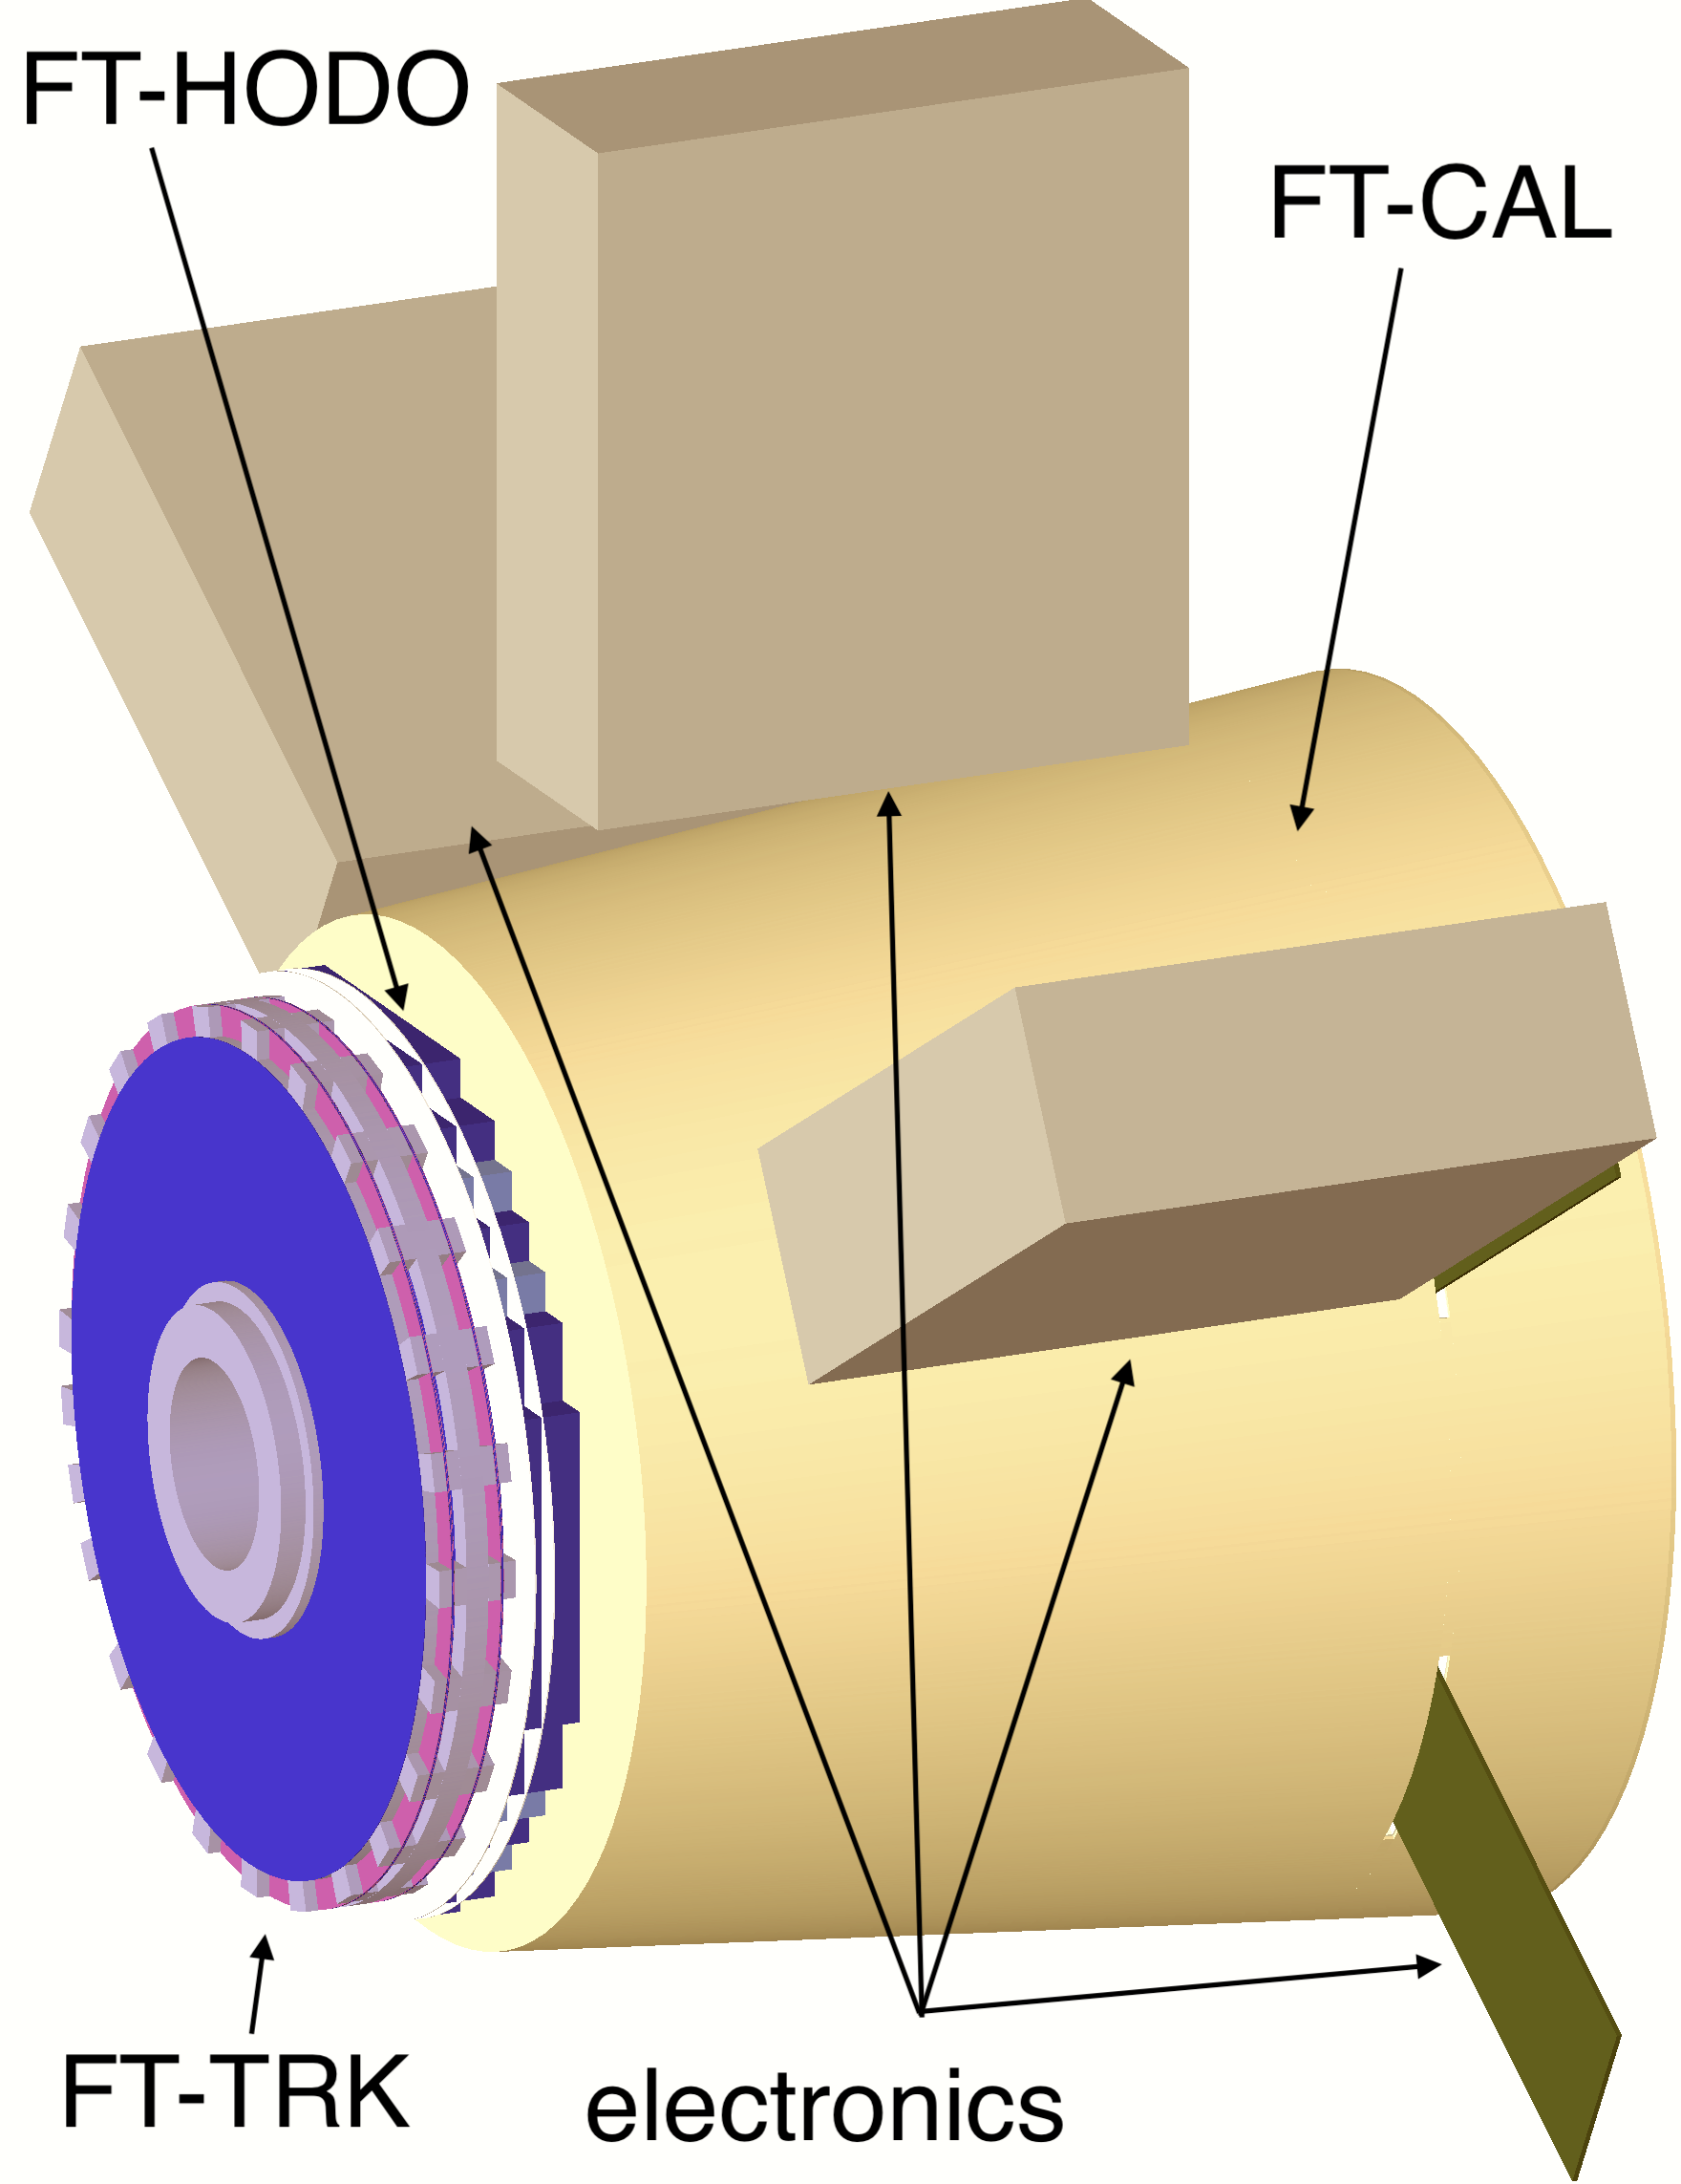
\includegraphics[width=0.99\columnwidth,keepaspectratio]{img/ftGeometry.png}
	\caption{The three detectors in the FT geometry implementation in GEMC.
             The disks form the micromegas tracker (FT-TRK). The hodoscope (FT-HODO) crystals are the boxes just behind the tracker,
			 while the calorimeter (FT-CAL) is encompassed in the cone. The volumes surrounding (FT-CAL) contain the electronics.}
	\label{fig:ftGeometry}
\end{figure}

For FTCal hits, the energy deposited is converted first to the charge produced at the end of the electronics chain composed
by the photosensor (APD) and pre-amplifier, and then to ADC.
The first conversion is based on the measured charge for cosmic rays that deposit a known energy in the crystals,
while the second conversion is based on the FADC conversion factor. A smearing on the final ADC values is added,
accounting for the Poisson distribution of photo-electrons produced by the photosensor, the Gaussian noise of the
photosensor and of the preamplifier. All parameters, the number of photo-electrons per MeV of energy deposited,
the RMS width of the APD noise, and of the preamplifier input noise, have been tuned to the experimental data.

The same approach is adopted to process FTHodo hits, in which the deposited energy is first converted to charge and then to ADC.
The smearing in this case accounts only for the Poisson distribution of the measured number of photo-electrons,
which dominates over other sources because of the relatively small number of photo-electrons per MeV of energy deposition.

The TDC of FTCal hits is computed from the time of the energy deposition, accounting for the speed of the scintillation light in
the crystal and the distance to the photosensor, assuming a known time-to-TDC conversion factor. A Gaussian smearing on the
resulting TDC is added based on a fixed RMS resoloution derived from the experimental measurements.

Similarly, the TDC of FTHodo hits is derived from the time of a given energy deposition, adding a fixed offset before the
conversion from time to TDC and a Gaussian smearing. As in previous cases, all relevant parameters have been tuned to the
observed detector response.

The digitized output bank variables are summarized in Table \ref{tab:ftBank}

\begin{table}[h]
	\begin{center}
		\begin{tabular}{| c | c | c |}
			\hline \hline
			Variable            & Description      \\
			\hline
		                         & Tracker         \\
			\hline
                         sector  &     sector      \\
                          layer  &      layer      \\
                      component  &  component      \\
                            ADC  &        ADC      \\
			\hline
		                         & Hodoscope       \\
			\hline
						 sector  &     sector      \\
                          layer  &      layer      \\
                      component  &  component      \\
                            ADC  &        ADC      \\
                            tdc  &        TDC      \\
			\hline
								 & Calorimeter     \\
			\hline
				         sector  &     sector      \\
				   	      layer  &      layer      \\
					  component  &  component      \\
							ADC  &        ADC      \\
							tdc  &        TDC      \\
			\hline \hline
		\end{tabular}
	\end{center}
	\caption{The digitized FT banks for the tracker, hodoscope and calorimeter}\label{tab:ftBank}
\end{table}

\noindent The time window  of the Tracker is set to to 132 ns: all geant4 steps within the same strip and time window will be collected on one hit.
The time window of the hodoscope and calorimeters are set to 400 ns: all geant4 steps within the same paddles and time window
will be collected on one hit in each system.

The FT hit process routines are: \url{https://github.com/gemc/source/blob/master/hitprocess/clas12/ft_cal_hitprocess.cc} and
\url{https://github.com/gemc/source/blob/master/hitprocess/clas12/ft_hodo_hitprocess.cc}.
